\documentclass[a4paper]{srs}

\hypersetup{%
	 pdftitle={RNA-Seqlyze SRS}%
	,pdfauthor={Patrick Pfeifer}%
	,pdfkeywords={thesis, rna-seq, srs}%
}

%\setcounter{tocdepth}{2}
%\setcounter{secnumdepth}{2}

\begin{document}
\begin{titlepage}
\begin{center}
%
% Logo & Project Name
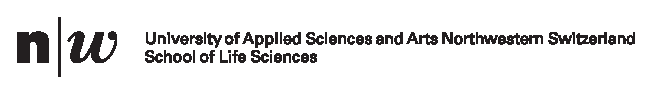
\includegraphics[width=0.4\textwidth]{../../assets/fhnw_hls_e_10mm}
\\[1cm]
{ \large Bachelor Thesis }
%
% Titel
\\[1cm]
{ \sffamily\Huge RNA-Seqlyze }
\\[1cm]
{ \sffamily\LARGE \bfseries Software Requirement Specification }
\\[2cm]
%
% Authors & Clients
\begin{minipage}{0.4\textwidth}
\begin{flushleft}
\large\emph{Student:}\\
	Patrick Pfeifer\\
\end{flushleft}
\end{minipage}
\begin{minipage}{0.4\textwidth}
\begin{flushright}
\large\emph{Professor:}\\
	Prof.~Dr.~Georg Lipps
\end{flushright}
\end{minipage}
%
% Verticall Fill
\vfill
%
% TODO'S
\listoftodos\vfill
%
% Version history
\setlength{\aboverulesep}{0pt}
\setlength{\belowrulesep}{0pt}
\setlength{\extrarowheight}{.75ex}
\begin{tabularx}{\textwidth}{|p{1.2cm}|>{\raggedright}X|X|p{3cm}|}
\rowcolor[gray]{0.8}
	Version & Author & Comment & Date\\
\midrule
	  0.1
	& Patrick Pfeifer
	& Initial draft version
	& 23. Mai 2012
\\
	  \ 
	& \ 
	& \ 
	& \ 
\\
\bottomrule
\end{tabularx}
\end{center}
\end{titlepage}

\tableofcontents
\newpage

	\section{Introduction}
\subsection{Purpose}
This document details the software requirements specification for the 
\nohyphenate{RNA-Seqlyze} next-generation RNA-sequencing analysis software. It 
defines the intended use of the software and lists the required features.

\subsection{Project Scope}
The RNA-Seqlyze web application is the main product of the RNA-Seqlyze free 
software project. The project was started by Patrick Pfeifer as part of his 
bachelor thesis at the University of Applied Sciences and Arts Northwestern 
Switzerland FHNW at the School of Life Sciences.

RNA-seq data is of increasing importance to the analysis of prokaryotes. The 
intended use of this software is to aid researchers in analyzing data generated 
by next-generation RNA sequencing methods (RNA-seq). Specifically, the software 
is supposed to improvement the annotation of existing genome data.

\subsection{Intended Audience and Structure of this Document}
All parties involved in the project may refer to this document as the definite
source of information concerning it.

Software users will generally be most interested in chapters number two and 
three. They contain information regarding the available features, with detailed
descriptions of the expected in- and outputs.

Developers planning to contribute code are strongly encouraged to read chapter
four as well, as it contains important information about the reliability-,
performance- and interface-requirements and -standards that must be fulfilled.

%\subsection{References}
%This document is written in adherence to the
%\emph{IEEE Recommended Practice for Software Requirements Specifications}:
%\begin{itemize}
%\item \href{http://standards.ieee.org/findstds/standard/830-1998.html}
%	{IEEE Std 830-1998\\
%	\url{http://standards.ieee.org/findstds/standard/830-1998.html}}
%\end{itemize}

	\section{Overall Description}

\subsection{Product Environment}

RNA-seq - the application of next-generation deep sequencing methods to DNA
transcripts - carries the potential to deliver new insights into the
organization and functionality of an organisms genome.

To achieve this, the large amounts of data produced by one of the various next
generation sequencing (NGS) platforms available on the market, have to be
analyzed in detail. Short reads of only a few dozen base pairs (bp) have to
mapped to a reference genome. The total number of reads mapped at each position
in the genome is counted to produce a transcript coverage "signal". The deeper
the coverage, the stronger, roughly, the gene is expressed in the organism.

\subsection{Product Features}

The envisioned web application is supposed to automate the process of analyzing
the data generated by NGS platforms deployed for RNA-seq experiments with
prokaryotes. The data will be made available to the application in FASTQ
or SRA format. In case SAM/BAM or coverage data files have already been
produced, they can be made available to the application as well.

The RNA-Seqlyze software processes this data using a novel algorithm.
It generates a list of transcribed sequences and assigns a confidence score to
each of those regions. The score will be computed based on the provided input
data as well as various other relevant information relating to the studied
organism. This auxiliary data incorporated into the processing algorithms has
been collected beforehand and is readily available to the application.
Specifically, the application will include predictions for shine-dalgarno
sequences, rho-independent terminators, operons (polycistronic transcripts) and,
optionally, promoter sites.

\subsection{User Characteristics}
It is assumed that a researcher using the application has basic
IT-skills and is used to interacting with popular computer interfaces.
The handling of the the RNA-Seqlyze web application shall be easy for him.

He has a good understanding of the technology applied to generate the data that
he wishes to analyze. A fair amount of specialized knowledge and fluency with
the most popular technical terms \emph{will be required} to use the application
in an efficient manner.

	\section{System Features}

\subsection{Priorities}

\vbox{
The priorities are assigned by the client and have the following meanings:\\

\begin{tabularx}{\textwidth}{lX}
	  high
	& This feature is indispensable and absolutely necessary for the 
	  correct functioning of the product. It must be implemented.
\\[1mm]
	  medium
	& This feature is not indispensable but makes a substantial 
	  contribution to the usability of the product. It should be implemented.
%\\[1mm]
%	  low
%	& This feature contributes towards a better usability of the product 
%	  but it is not a strictly necessity. The functionality would be nice to 
%	  have.
\end{tabularx}
}

\subsection{RNA-seq Data Analysis}

\subsubsection*{Description and Priority}
TBD
\\Priority: {\bfseries high}
\subsubsection*{Functional Requirements}
TBD

\subsection{Custom Track Generation}

\subsubsection*{Description and Priority}
TBD
\\Priority: {\bfseries medium}
\subsubsection*{Functional Requirements}
TBD

	\section{Nonfunctional Requirements}

\subsection{Quality Requirements}

\subsubsection{Documentation}
The source code shall be documented, such that modifications or additional 
modules could be integrated by third-party developers. Furthermore, an
extensive user manual shall be composed.

\subsubsection{Usability}
The application's user interface shall be easy to use and follow current 
conventions. When using the software, the user shall constantly be informed what 
the current state of the application is, which steps have been already carried 
out and which ones are to be carried out next.

\subsubsection{Reliability and Maintainability}
An error-free execution of all functions of the software shall be achieved by 
writing tests for all parts (unit tests) as well as for the whole system 
(integration tests). The coverage of the unit tests shall reach at least 80 
Percent of the source code.

In case the server hosting the application is rebooted, the application shall be 
automatically restarted as well.

\subsubsection{Performance and Efficiency}
Load times and data transmission shall be within reasonable bounds. Except for 
the transmission of big data files from the users PC to the application server, 
there shall be no significant delays when using the application.

The time required to process a given dataset shall be estimated and the estimate 
shall be presented to the user before he triggers the processing by clicking the 
designated button.

\subsubsection{Security}
The data transmitted to the application for processing is not expected to 
be privacy-sensitive or confidential. Data submitted by individual users will 
generally not be presented to other users, but no efforts are made to protect 
the data from being retrieved by other authorized users of the server.

\subsection{Interface Requirements}

TBD

	\section{Appendices}

\subsection{Glossary}

\begin{tabularx}{\textwidth}{lX}
	  RNA-seq
	& NGS Technology applied to whole genome transcriptome profiling
\\
\end{tabularx}

\end{document}

% vim: tw=80:fo+=w
